\subsection{Period 4: Reappearance of a new detached haze layer around the Summer Solstice (2015-2017) - $L_s=\ang{75}-\ang{95}$}

The first occurrence of the detached haze in this period is the 3$^{rd}$ December 2015
(Fig.~\ref{fig:dhl_2015_2017}a). Strictly speaking, it
does not differ from the previous sporadic detached haze layers observed in the period 2012-2015. But, after
this observation, the detached haze was present in each observation. The detached haze became stable in time,
similarly to the detached haze before the equinox. Therefore, we consider this date as the beginning of the
reappearance of the detached haze ($L_s=\ang{74}$). The evolution of the haze during this period is displayed in
Fig.~\ref{fig:dhl_2015_2017}. These observations validate the long awaited reappearance of the detached haze layer,
just before the end of the Cassini mission in September 2017.

\begin{figure*}[!ht]
    \centering
    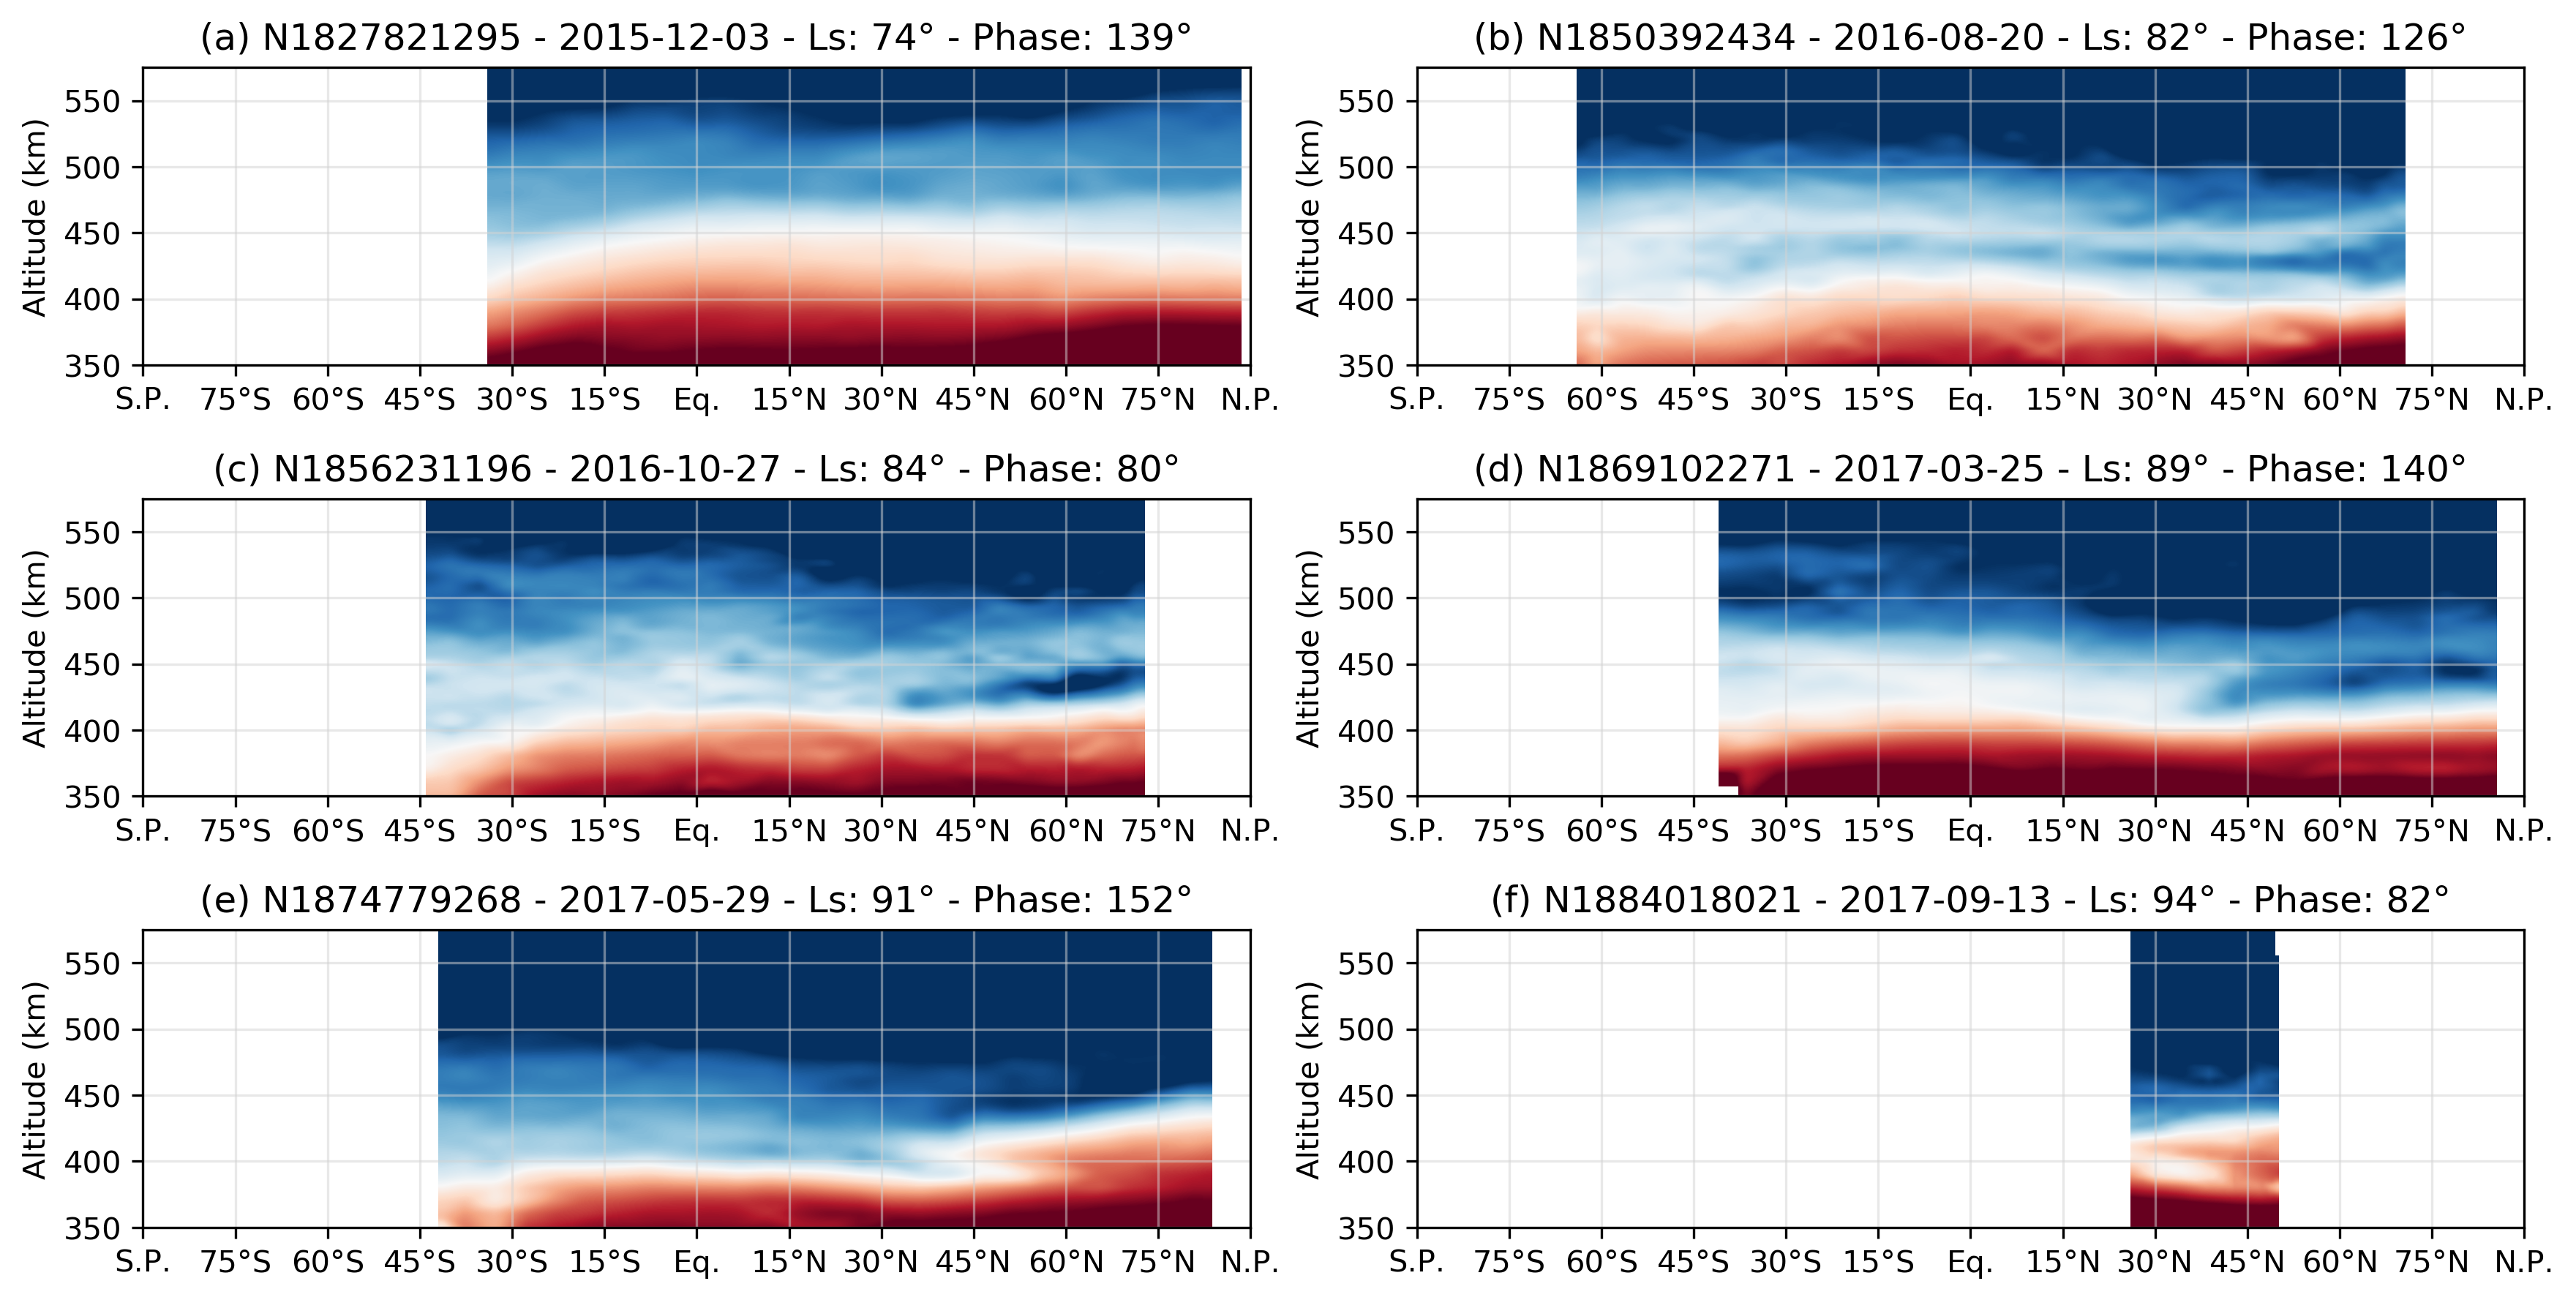
\includegraphics[width=\textwidth]{Fig/Lat_beta-2015_2017.png}
    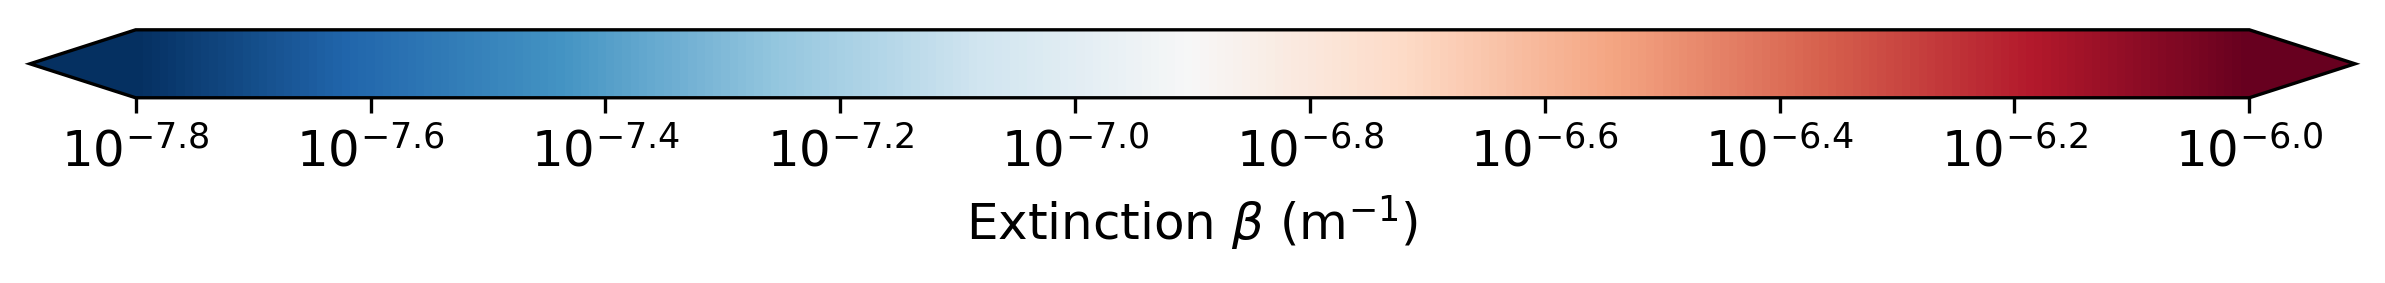
\includegraphics[width=.5\textwidth]{Fig/Extinction_colorbar.png}\vspace{-.3cm}
    \caption{Same as the figures~\ref{fig:dhl_2004_2008}, \ref{fig:dhl_2008_2012}
    and~\ref{fig:dhl_2012_2015} for 6 images taken between 2015 and 2017
    ($L_s=\ang{75}-\ang{95}$) during the reappearance of the DHL.
    The image \textbf{N1884018021\_1} is one of the very last observation of Titan before
    the end of the Cassini mission in September 2017.}
    \label{fig:dhl_2015_2017}
\end{figure*}

The detached haze layer is not very well defined but it can be perceived at all latitudes
around 490 - 520 km (Fig.~\ref{fig:dhl_2015_2017}a). We notice a contraction
the main haze, with the top of the haze dropped by 50 km in January 2016 compared to October 2015
(Fig.~\ref{fig:dhl_2012_2015}d). The main elements of the reappearance (altitude and date) confirms the
predictions made by the general circulation models \citep{Lebonnois2012,Larson2015} and the prediction
reported in \cite{West2011}. The detailed comparison between the observations and GCM is discussed further
in section 5.

With time, the detached haze layer is better marked and the zone of depletion is more pronounced, especially in the
northern hemisphere (Fig.~\ref{fig:dhl_2015_2017}b). The situation seems to be analogue to an early stage of
the structure observed in 2004 (Fig~\ref{fig:dhl_2004_2008}a, with the opposite latitude).
However, although the detached haze persists in time,
it also settles and almost merges with the main haze in October 2016 (Fig.~\ref{fig:dhl_2015_2017}c).
In the  following observations (Figs.~\ref{fig:dhl_2015_2017}d and e), we are
witnessing the complex evolution of the first appeared detached haze that merge with the main layer at latitude southward
of \ang{35}N while it remains stable around 450 km northward to \ang{35}N and seems to vanish in May 2017 rather than settle.
This structure was still observed in the very last image of Titan taken by Cassini just before its final plunge into Saturn
atmosphere (Fig.~\ref{fig:dhl_2015_2017}f) in September 2017.

A secondary detached haze layer appears in October 2016 in the southern hemisphere at high altitude around 520 km
(Fig.~\ref{fig:dhl_2015_2017}c). Its northern boundary is not well defined. This new structure will be persistent with
time, at planetary scale up to the end of Cassini mission but is gradually descending. The results reported by \cite{West2018}
concerns the detached haze at equator only. Although they already revealed a complex behavior of the detached haze layer, the
present observations show a dichotomy between the two hemispheres. The detail of the evolution, the split in a double layer
structure, the formation and disappearance of several structures was completely unexpected. According to GCMs, six years
after equinox, the post-equinoctial circulation was supposed to be already installed with a planetary scale circulation cell
from the south hemisphere to the north polar region. Apparently, this is not the case in the observations.

These observations from 2004 to 2017 does not completely cover half a Titan year. The first and last observations
were taken almost at the opposite season, $L_s=\ang{297}$ and \ang{94} respectively (\emph{i.e.} \ang{157} apart).
This prevents direct comparisons between the detached haze at the beginning and at the end of the mission,
although in both cases they are taken more than a season after the previous solstice.
